% ex: ts=2 sw=2 sts=2 et filetype=tex
% SPDX-License-Identifier: CC-BY-SA-4.0

\section{Introducción e instalación}

\begin{frame}[c]{¿Qué es Matplotlib?}
  \begin{itemize}
    \item Matplotlib es una biblioteca de trazado de gráficos de bajo
          nivel en Python que sirve como utilidad de visualización.
    \pausa
    \item Matplotlib fue creado por John D. Hunter.
    \pausa
    \item Matplotlib es de código abierto y podemos usarlo libremente.
    \pausa
    \item Matplotlib está escrito principalmente en Python, algunos
          segmentos están escritos en C, Objective-C y Javascript
          para compatibilidad con la plataforma.
  \end{itemize}
\end{frame}

\begin{frame}[c]{¿Dónde está el código base de Matplotlib?}
  \begin{itemize}
    \item El código fuente de Matplotlib se encuentra en este
      repositorio de github
      \href{https://github.com/matplotlib/matplotlib}
      {https://github.com/matplotlib/matplotlib}
  \end{itemize}
\end{frame}

\begin{frame}[fragile]
  \frametitle{Instalación de Matplotlib}
    Si ya tiene Python y PIP instalados en un sistema,
    entonces la instalación de Matplotlib es muy fácil.

  \begin{exampleblock}{Ejemplo:}
    Instálalo usando este comando:
    \begin{lstlisting}[language=Python]
C:\Users\Your Name>pip install matplotlib 
    \end{lstlisting}
  \end{exampleblock}
  Si este comando falla, utilice una distribución de Python que
  ya tenga Matplotlib instalado, como Anaconda, Spyder, etc.
\end{frame}

\begin{frame}[fragile]
  \frametitle{Importar Matplotlib}
    Una vez instalado Matplotlib, impórtelo en sus aplicaciones
    agregando la declaración: \textbf{import module}
  \begin{exampleblock}{Ejemplo:}
    \begin{lstlisting}[language=Python]
import matplotlib
    \end{lstlisting}
  \end{exampleblock}
  Ahora Matplotlib está importado y listo para usar
\end{frame}

\begin{frame}[fragile]
  \frametitle{Comprobación de la versión de Matplotlib}

  La cadena de versión se almacena en \textbf{\_\_version\_\_} el atributo.

  \begin{exampleblock}{Ejemplo:}
    \begin{lstlisting}[language=Python]
import matplotlib

print(matplotlib.__version__)
    \end{lstlisting}
  \end{exampleblock}
  \begin{block}{Nota:}
    Se utilizan dos caracteres de subrayado en \textbf{\_\_version\_\_}.
  \end{block}
\end{frame}

\section{Gráficos con Pyplot}

\begin{frame}[fragile]
  \frametitle{Pyplot}

  La mayoría de las utilidades de Matplotlib se encuentran
  bajo el submódulo \textbf{pyplot} y normalmente se importan
  bajo el alias \textbf{plt}:

  \begin{exampleblock}{Ejemplo:}
    \begin{lstlisting}[language=Python]
import matplotlib.pyplot as plt 
    \end{lstlisting}
  \end{exampleblock}
  Ahora el paquete Pyplot puede denominarse plt.
\end{frame}

\begin{frame}[fragile]
  \frametitle{Pyplot}

  \begin{columns}
      \column{0.5\textwidth}
        \begin{exampleblock}{Ejemplo:}
          Dibuje una línea en un diagrama desde la posición
          (0,0) hasta la posición (6,250):
          \lstinputlisting{ejemplos/e01.py}
        \end{exampleblock}
      \column{0.5\textwidth}
      \begin{center}
          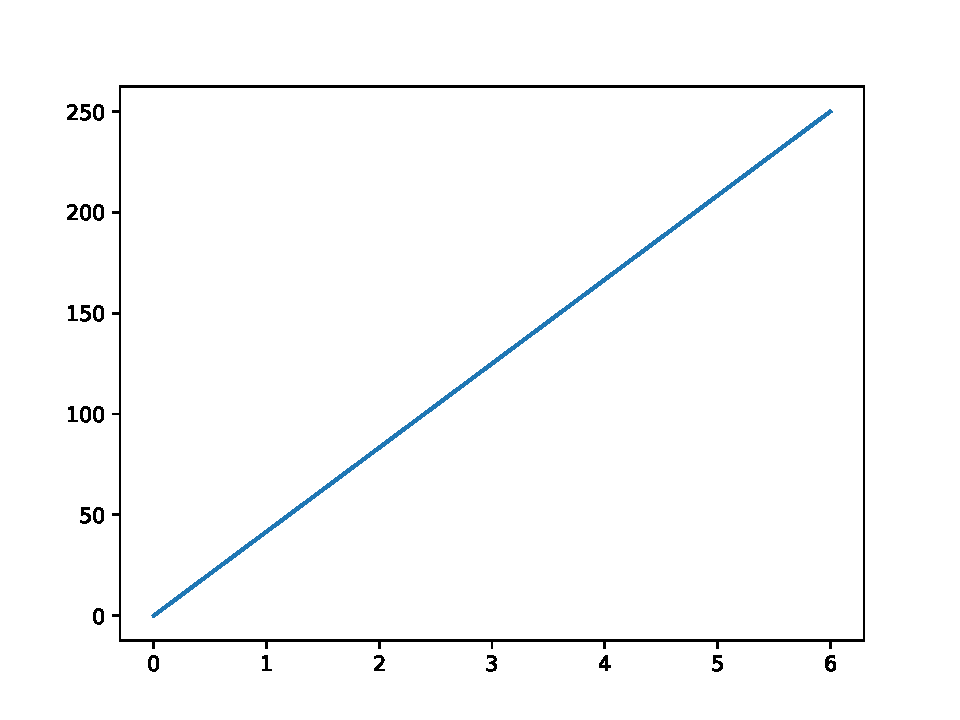
\includegraphics[scale=0.5]{ejemplos/e01.pdf}
      \end{center}
  \end{columns}
\end{frame}

\begin{frame}[fragile]
  \frametitle{}

  \begin{exampleblock}{Ejemplo:}
    \begin{lstlisting}[language=Python]
    \end{lstlisting}
  \end{exampleblock}
\end{frame}

\begin{frame}[fragile]
  \frametitle{}

  \begin{exampleblock}{Ejemplo:}
    \begin{lstlisting}[language=Python]
    \end{lstlisting}
  \end{exampleblock}
\end{frame}
